\documentclass[
  bibliography=totoc,     % Literatur im Inhaltsverzeichnis
  captions=tableheading,  % Tabellenüberschriften
  titlepage=firstiscover, % Titelseite ist Deckblatt
]{scrartcl}


%Damit neue Paragraphen nicht eingerückt sind
\setlength\parindent{0pt}

%Für Farbige Formel 
\usepackage{color} 
\usepackage[dvipsnames]{xcolor}
%Damit die Bildcaptions nicht so groß sind 
\usepackage{caption}
\captionsetup[wrapfigure]{font=footnotesize}

% Paket float verbessern
\usepackage{scrhack}

% Warnung, falls nochmal kompiliert werden muss
\usepackage[aux]{rerunfilecheck}

% unverzichtbare Mathe-Befehle
\usepackage{amsmath}
% viele Mathe-Symbole
\usepackage{amssymb}
% Erweiterungen für amsmath
\usepackage{mathtools}

% Fonteinstellungen
\usepackage{fontspec}
% Latin Modern Fonts werden automatisch geladen
% Alternativ zum Beispiel:
%\setromanfont{Libertinus Serif}
%\setsansfont{Libertinus Sans}
%\setmonofont{Libertinus Mono}

% Wenn man andere Schriftarten gesetzt hat,
% sollte man das Seiten-Layout neu berechnen lassen
\recalctypearea{}

% deutsche Spracheinstellungen
\usepackage[ngerman]{babel}
% \usepackage[american]{babel}  % englische Einstellungen


\usepackage[
  math-style=ISO,    % ┐
  bold-style=ISO,    % │
  sans-style=italic, % │ ISO-Standard folgen
  nabla=upright,     % │
  partial=upright,   % │
  mathrm=sym,        % ┘
  warnings-off={           % ┐
    mathtools-colon,       % │ unnötige Warnungen ausschalten
    mathtools-overbracket, % │
  },                       % ┘
]{unicode-math}

% traditionelle Fonts für Mathematik
\setmathfont{Latin Modern Math}
% Alternativ zum Beispiel:
%\setmathfont{Libertinus Math}

\setmathfont{XITS Math}[range={scr, bfscr}]
\setmathfont{XITS Math}[range={cal, bfcal}, StylisticSet=1]

% Zahlen und Einheiten
\usepackage[
  locale=DE,                   % deutsche Einstellungen
  % locae=US,                    % englische Einstellungen
  separate-uncertainty=true,   % immer Unsicherheit mit \pm
  per-mode=symbol-or-fraction, % / in inline math, fraction in display math
]{siunitx}

% chemische Formeln
\usepackage[
  version=4,
  math-greek=default, % ┐ mit unicode-math zusammenarbeiten
  text-greek=default, % ┘
]{mhchem}

% richtige Anführungszeichen
\usepackage[autostyle]{csquotes}

% schöne Brüche im Text
\usepackage{xfrac}

% Standardplatzierung für Floats einstellen
\usepackage{float}
\floatplacement{figure}{htbp}
\floatplacement{table}{htbp}

%um Text neben Bild darzustellen 
\usepackage{wrapfig}

% Floats innerhalb einer Section halten
\usepackage[
  section, % Floats innerhalb der Section halten
  below,   % unterhalb der Section aber auf der selben Seite ist ok
]{placeins}

% Seite drehen für breite Tabellen: landscape Umgebung
\usepackage{pdflscape}

% Captions schöner machen.
\usepackage[
  labelfont=bf,        % Tabelle x: Abbildung y: ist jetzt fett
  font=small,          % Schrift etwas kleiner als Dokument
  width=0.9\textwidth, % maximale Breite einer Caption schmaler
]{caption}
% subfigure, subtable, subref
\usepackage{subcaption}

% Grafiken können eingebunden werden
\usepackage{graphicx}

% schöne Tabellen
\usepackage{booktabs}

% Verbesserungen am Schriftbild
\usepackage{microtype}

% Literaturverzeichnis
\usepackage[ natbib=true, style=numeric,sorting=none]{biblatex}
%\usepackage[
 % backend=biber,
%]{biblatex}
% Quellendatenbank
\addbibresource{lit.bib}
\addbibresource{programme.bib}

% Hyperlinks im Dokument
\usepackage[
  german,
  unicode,        % Unicode in PDF-Attributen erlauben
  pdfusetitle,    % Titel, Autoren und Datum als PDF-Attribute
  pdfcreator={},  % ┐ PDF-Attribute säubern
  pdfproducer={}, % ┘
]{hyperref}
% erweiterte Bookmarks im PDF
\usepackage{bookmark}

% Trennung von Wörtern mit Strichen
\usepackage[shortcuts]{extdash}

%selber hinzugefügt
\usepackage{tabularray}
\UseTblrLibrary{booktabs}

\author{%
  Amelie Hater\\%
  \href{mailto:amelie.hater@tu-dortmund.de}{amelie.hater@tu-dortmund.de}%
  \and%
  Ngoc Le\\%
  \href{mailto:ngoc.le@tu-dortmund.de}{ngoc.le@tu-dortmund.de}%
}
\publishers{TU Dortmund – Fakultät Physik}

\subject{V48}
\title{Dipolrelaxation in Ionenkristallen}
% \date{%
%   Durchführung: DATUM
%   \hspace{3em}
%   Abgabe: DATUM
% }
\date{%
\begin{tabular}{l l}
  Durchführung: & 16.06.2025 \\
  Abgabe: & 26.06.2025 \\
  Korrektur: & 11.07.2025 \\
\end{tabular}
}

\begin{document}

\maketitle
\thispagestyle{empty}
\tableofcontents
\newpage

\section{Zielsetzung}
\label{sec:Zielsetzung}

\section{Theorie}
\label{sec:Theorie}
\cite{anleitungV48} 
\cite{IonicThermo}
\cite{Irradiation}
\cite{Bunsengesellschaft}
\cite{Fuller}
% \subsection{Vorbereitungsaufgaben}
% \label{sec:Vorbereitungsaufgaben}

\section{Experimental setup and measurements}
\label{sec:Experimentale}
The experiment is conducted by using the Sagnac-Interferometer introduced in \ref{subsec:Sagnac_Interferometer}. 
The topology of the interferometer can be seen in \autoref{pic:Sagnac-Interferometer}.As a 
source of light a Helium-Neon laser is used. The plane of the linear polarized laser beam is tilted about $45°$ in comparison to 
the vertical. This leads to the beam being split into two beams of the same intensity and perpendicular polarization by the PBSC.
In front of the PBSC a polarisation filter is placed so the incomming beam is traveling through the filter and afterwards through the 
PBSC. 

\begin{figure}
    \centering
    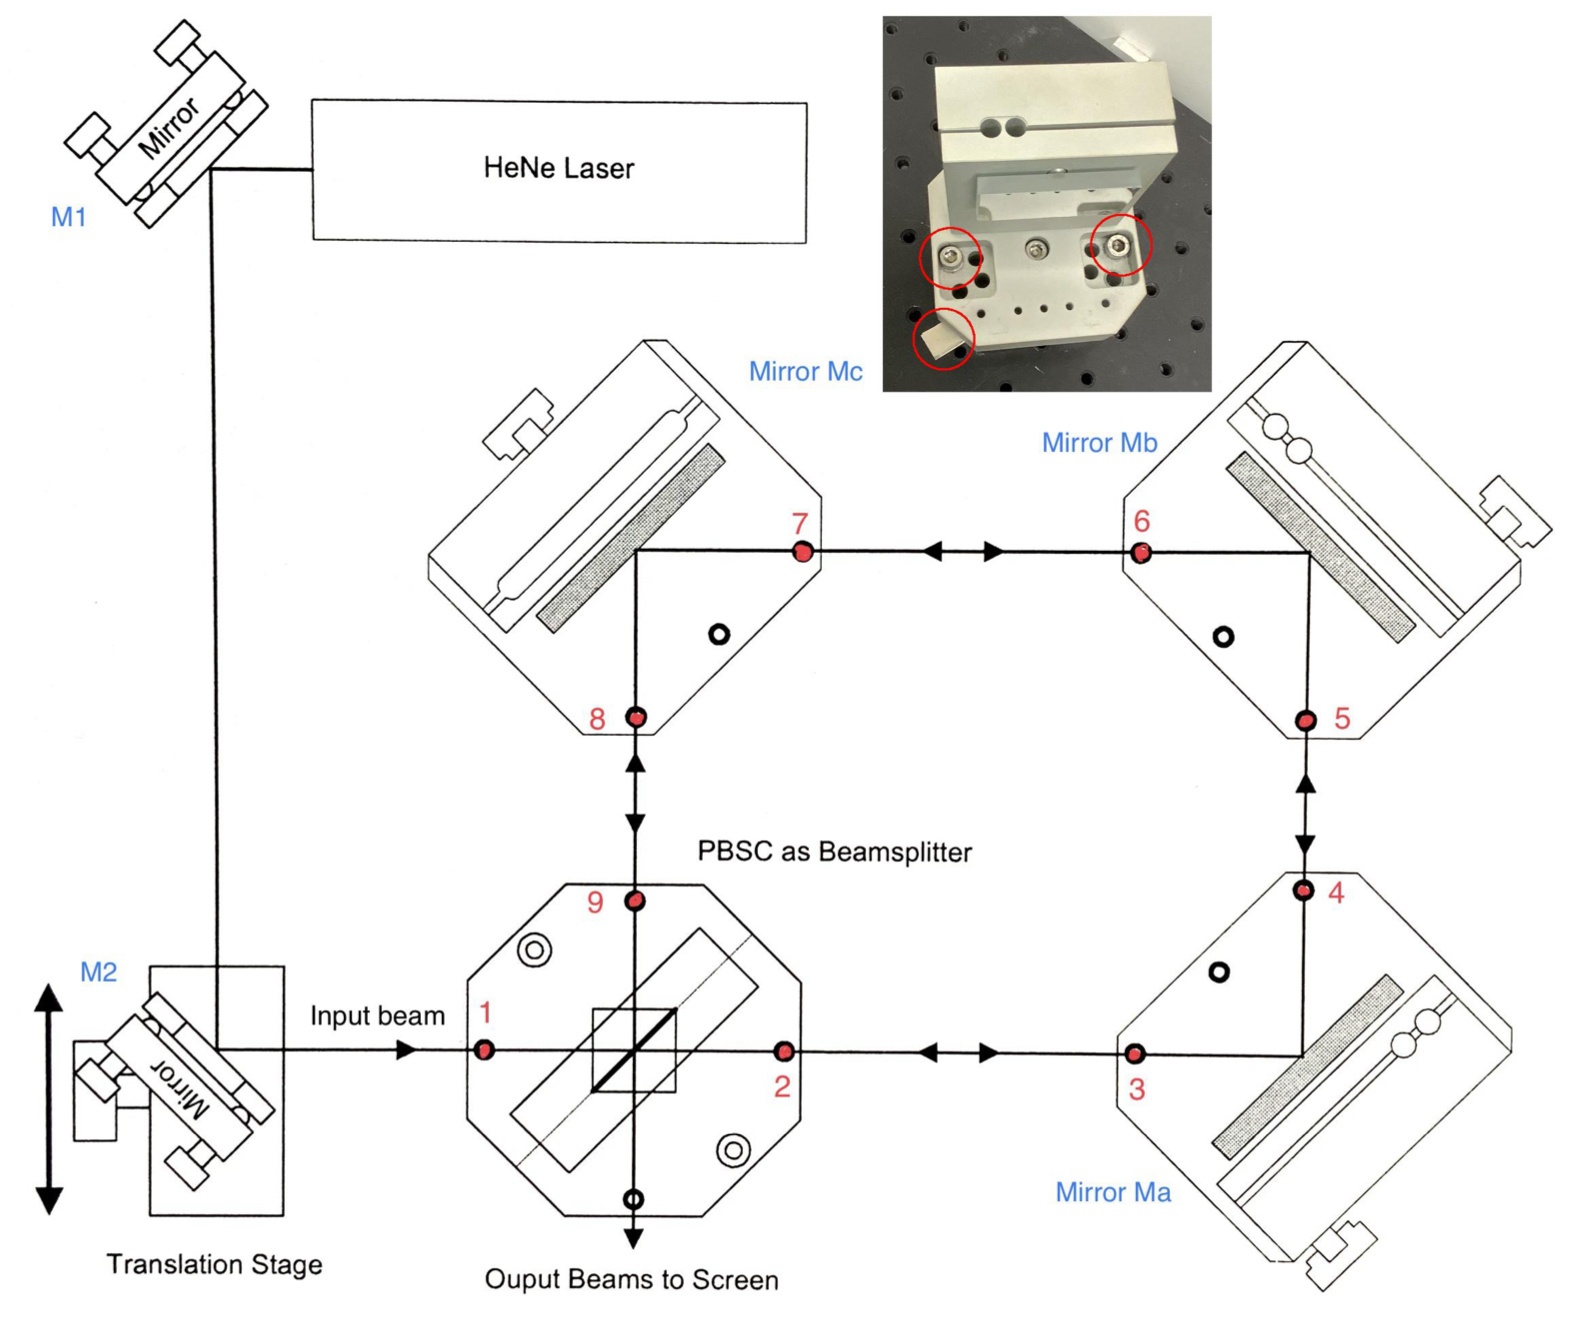
\includegraphics[width=0.70\textwidth]{content/Bilder/Sagnac_Interferometer.jpeg}
    \caption{Topology of the Sagnac-Interferometer}
    \label{pic:Sagnac-Interferometer}
  \end{figure}

To make the interference of the two beams possible the beams must travel through a polarization filter to create an overlapping polarization. 

\subsection{Alignment}
The correct alignment is a critical part of the experiment. For the interference to work the beams have to be parallel to each over and 
overlap at all times. This is achieved by using adjustment plated which have holes at the top where the beam should travel through. 

% systematische Messfehler von T \pm 1 K und I \pm 0.01e-11 bzw \pm0.01e-10 nicht vergessen zu erwähnen! 
\section{Auswertung}
\label{sec:Auswertung}
Die aufgenommenen Messwerte der beiden Messreihen sind in \autoref{tab:Messung1} und \autoref{tab:Messung2} aufgelistet. Bei der zweiten Messreihe sind einige Vorzeichen eingeklammert. Die Erklärung dazu folgt in Abschnitt \ref{sec:Untergrundkorrektur}.
\subsection{Bestimmung der Heizraten}
\label{sec:Heizraten}
% Heizraten:
% Erste Messung
% (Heizrate) m1: 0.855+/-0.013 K/min bzw. 0.01425+/-0.00022 K/sec
% b1: 210.1+/-0.8 K
% Zweite Messung
% (Heizrate) m2: 2.650+/-0.032 K/min bzw. 0.0442+/-0.0005 K/sec
% b2: 195.1+/-0.7 K
\begin{figure}
  \centering
  \includegraphics[width=0.8\linewidth]{build/Heizraten.pdf}
  \caption{Gemessene Temperatur gegen die Zeit der beiden Messreihen und eine lineare Regression zur Bestimmung der Heizraten.}
  \label{fig:Heizraten}
\end{figure}
Für die Berechnung der Relaxationszeit in Abschnitt \ref{sec:AuswertungRelaxationszeit} wird die Heizrate benötigt.
Daher ist in der \autoref{fig:Heizraten} die gemessene Temperatur der beiden Messreihen gegen die Zeit aufgetragen.
Mithilfe einer linearen Regression der Form 
$$
T(t) = \alpha \cdot t + \beta
$$
werden die Heizraten bestimmt, die den Steigungen $m$ entsprechen. 
Somit ergeben sich die folgenden Parameter
\begin{align*}
    \alpha_1 = \SI{0.855\pm0.013}{\kelvin\per\minute} = \SI{0.01425\pm0.00022}{\kelvin\per\second}\text{ und }\beta_1= \SI{210.1\pm0.8}{\kelvin}\\
    \alpha_2 = \SI{2.650\pm0.032}{\kelvin\per\minute} = \SI{0.0442\pm0.0005}{\kelvin\per\second}\text{ und }\beta_1= \SI{195.1\pm0.7}{\kelvin}\,.
\end{align*}
\FloatBarrier
\subsection{Untergrundkorrektur und Auswahl gültiger Messdaten}
\label{sec:Untergrundkorrektur}
Die gemessenen Ströme $I$ in Abhängigkeit der Temperatur $K$ sind für beide Messreihen in \autoref{fig:Untergrund1} und \autoref{fig:Untergrund2} abgebildet.
Zusätzlich ist in den Abbildungen markiert, welche Messwerte für die weitere Auswertung ausgeschlossen und welche zur Bestimmung des Untergrunds verwendet werden.
Eine Korrektur des Untergrunds ist erforderlich, weil der gemessene Gesamtstrom neben dem Depolarisationsstrom auch Beiträge aus anderen Prozessen enthält. Solche Prozesse sind bspw. thermisch aktivierte Ströme. 
Da diese Stromanteile nicht im direkten Zusammenhang mit der Relaxation der Dipole stehen, würde eine Berücksichtigung dieser Anteile zu systematischen Fehlern in der Bestimmung der Aktivierungsenergie und Relaxationszeit führen. 
Als Untergrund werden hier die Messwerte identifiziert, die in Temperaturbereichen außerhalb des Relaxationspeaks liegen. 
In diesem Bereichen ist der Einfluss des Depolarisationsstroms vernachlässigbar, und der gemessene Strom folgt näherungsweise einem exponentiellen Temperaturverhalten.
Zur Modellierung des Untergrunds wird daher ein exponentieller Fit der Form 
$$
I_U = \alpha \cdot \exp(\beta\cdot T) + \gamma
$$
verwendet. 
Die exkludierte Messdaten werden im weiteren Verlauf der Auswertung nicht berücksichtigt, da sie keinem eindeutigen physikalischen Beitrag zugeordnert werden konnten und somit die weitere Auswertung verfälschen würde. 
Für die zweite Messreihe werden zusätzlich Messwerte innerhalb des Depolarisationspeaks vernachlässigt, da diese deutlich vom charakteristischen Verlauf abweichen, wie es z.B. in der \autoref{fig:Untergrund1} abbgebildet ist.
Die Originaldaten der zweiten Messreihe sind in \autoref{fig:Untergrund2_f} dargestellt. 
Im Vergleich zur ersten Messreihe in \autoref{fig:Untergrund1} fällt auf, dass der Verlauf nicht dem erwarteten Verhalten eines Depolarisationsstroms entspricht. 
Es wird daher vermutet, dass die Vorzeichen der Messwerte ab dem Punkt, an dem die Größenordnung des gemessenen Stroms wechselt, nicht korrekt dokumentiert wurden. Diese Vorzeichen sind daher in \autoref{tab:Messung2} eingeklammert.
Durch eine entsprechende Korrektur der Vorzeichen ergibt sich der in \autoref{fig:Untergrund2} dargestellte Verlauf, die dem erwarteten Verhalten entspricht. Daher wird diese korrigierte Version für die weitere Auswertung verwendet.\\
Aus der Ausgleichsfunktion der ersten Messreihe ergibt sich eine Untergrundfunktion von 
\begin{align*}
    I_{U,1} = \SI{2.9\pm2.2}{\micro\ampere}\cdot \exp\left(\SI{0.0495\pm0.0028}{\per\kelvin}\cdot T \right) - \SI{0.76\pm0.04}{\pico\ampere}\,.
\end{align*}
\begin{figure}
    \centering
    \includegraphics[width=0.8\linewidth]{build/ersterStrom.pdf}
    \caption{Gemessene Daten der ersten Messreihe sowie einem Fit des Untergrunds mit exponentiellen Ansatz.}
    \label{fig:Untergrund1}
\end{figure}
% Erste Messreihe: m1_exp: (2.9+/-2.2)e-06 a1_exp: 0.0495+/-0.0028 b1_exp: -0.76+/-0.04
\begin{figure}[t]
    \centering
    \includegraphics[width=0.8\linewidth]{build/zweiterStromVor.pdf}
    \caption{Gemessene Daten der zweiten Messreihe (nach Vorzeichen Korrektur) sowie einem Fit des Untergrunds mit exponentiellen Ansatz.}
    \label{fig:Untergrund2}
\end{figure}
\begin{figure}
    \centering
    \includegraphics[width=0.8\linewidth]{build/zweiterStrom.pdf}
    \caption{Gemessene Daten der zweiten Messreihe (vor Vorzeichen Korrektur).}
    \label{fig:Untergrund2_f}
\end{figure}
% Zweite Messreihe: m2_exp: 0.00011+/-0.00011 a2_exp: 0.040+/-0.004 b2_exp: -1.29+/-0.12
Die Ausgleichsfunktion der zweiten Messreihe sieht wie folgt aus:
\begin{align*}
    I_{U,2} = \SI{0.00011\pm0.00011}{\ampere}\cdot \exp\left(\SI{0.040\pm0.004}{\per\kelvin}\cdot T \right) - \SI{1.29\pm0.12}{\pico\ampere}\,.
\end{align*}
\FloatBarrier
Die Untergrundfunktionen werden von den jeweiligen Messreihen abgezogen, somit ergeben sich die in \autoref{fig:Untergrundfrei1} und \autoref{fig:Untergrundfrei2} dargesetellten Messdaten. 
In diesen Abbildungen sind die ausgeschlossenen Messwerte bereites herausgefiltert. 
Zudem sind die Messwerte gekennzeichnet, die für die Bestimmung der Aktivierungsenergie verwendet werden.
Hierfür wird einmal die Methode mit dem Polarisationsansatz und einmal mit dem Stromdichtenansatz gewählt.
Die genaue Anwendung der beiden Ansätze wird in den folgenden beiden Abschnitten erläutert.
\begin{figure}
    \centering
    \includegraphics[width=0.8\linewidth]{build/ersterUntergrundfrei.pdf}
    \caption{Korrigierte Messdaten der ersten Messreihe mit Kennzeichnung der verwendeten Messdaten für die zwei Methoden zur Bestimmung der Aktivierungsenergie.}
    \label{fig:Untergrundfrei1}
\end{figure}

\begin{figure}
    \centering
    \includegraphics[width=0.8\linewidth]{build/zweiterUntergrundfrei.pdf}
    \caption{Korrigierte Messdaten der zweiten Messreihe mit Kennzeichnung der verwendeten Messdaten für die zwei Methoden zur Bestimmung der Aktivierungsenergie.}
    \label{fig:Untergrundfrei2}
\end{figure}

\FloatBarrier
\subsection{Berechnung der Aktivierungsenergie mit Polarisationsansatz}
% Polarisationsansatz
% Messung 1
% m1_pol: (-8.66+/-0.23)e+03 K
% b1_pol: 36.6+/-1.0 ohne Einheit
% W1_pol = (1.196+/-0.032)e-19 eV
Der Polarisationsansatz basiert auf Gleichung \ref{eqn:approx_kalte_Temperaturen}. Auf Grundlage dieser Beziehung werden aus den Messreihen die Datenpunkte entnommen, die einem exponentiellen Verlauf folgen. 
Durch Anwendung des natürlichen Logarithmus auf diese Messwerte ergibt sich ein linearer Zusammenhang mit $T^{-1}$. 
Diese lineare Beziehung ist in \autoref{fig:Polarisation1} und \autoref{fig:Polarisation2} dargesetellt. Durch eine lineare Regression der Form
$$
\ln\left(\frac{I_D}{I_0}\right) = \alpha^{\text{Pol.}} \cdot \frac{1}{T} +\beta^{\text{Pol.}}\;,
$$
mit $I_0 = \SI{1}{\pico\ampere}$, ergibt sich die Aktivierungsenergie $W$ aus der Steigung $\alpha$ über den Zusammenhang $W = -k_{\text{B}}\cdot \alpha^{\text{Pol.}}$.
\begin{figure}
    \centering
    \includegraphics[width=0.8\linewidth]{build/polarisation1.pdf}
    \caption{Messdaten sowie linearer Fit der ersten Messreihe zur Bestimmung der Aktivierungsenergie mithilfe des Polarisationsansatzes.}
    \label{fig:Polarisation1}
\end{figure}
Aus der linearen Regression ergeben sich für die erste Messreihe die Parameter
\begin{align*}
    \alpha_1^{\text{Pol.}} = -\left(8,66\pm0,23\right)\cdot 10^{-3}\,\si{\kelvin} \text{ und } \beta_1^{\text{Pol.}}=\SI{36.6\pm1.0}{}\,.
\end{align*}
Die entsprechende Aktivierungsenergie beträgt somit
\begin{align*}
    W_1^{\text{Pol.}} = \left(0,747 \pm 0,020\right)\,\si{\electronvolt}\,.
\end{align*}
% m1_pol: (-8.66+/-0.23)e+03 K
% b1_pol: 36.6+/-1.0 ohne Einheit$$
Für die zweite Messreihe ergeben sich die folgenden Parameter :
\begin{align*}
    \alpha_2^{\text{Pol.}} = -\left(7,5\pm0,23\right)\cdot 10^{-3}\,\si{\kelvin} \text{ und } \beta_2^{\text{Pol.}}=\SI{36\pm4}{}\,.
\end{align*}
Demnach ergibt sich eine Aktivierungsenergie von 
\begin{align*}
    W_2^{\text{Pol.}} = \left(0,65 \pm 0,08\right)\,\si{\electronvolt}\,.
\end{align*}
\begin{figure}
    \centering
    \includegraphics[width=0.8\linewidth]{build/polarisation2.pdf}
    \caption{Messdaten sowie linearer Fit der zweiten Messreihe zur Bestimmung der Aktivierungsenergie mithilfe des Polarisationsansatzes.}
    \label{fig:Polarisation2}
\end{figure}
% Messung 2
% m2_pol: (-7.5+/-0.9)e+03 K
% b2_pol: 31+/-4 ohne Einheit
% W2_pol = (1.04+/-0.12)e-19 eV
\FloatBarrier  
\subsection{Berechnung der Aktivierungsenergie mit Stromdichtenansatz}
\label{sec:AuswertungStromdichtenansatz}
% Stromdichtenansatz:
% erste Messung
% m1_str: (1.114+/-0.023)e+04 K
% b1_str: -42.2+/-0.9 keine Einheit
% W1_str = (1.538+/-0.032)e-19 eV
% zweite Messung
% m2_str: (1.05+/-0.05)e+04 K
% b2_str: -38.8+/-1.9 keine Einheit
% W2_str = (1.45+/-0.07)e-19 eV
Im Gegensatz zum Polarisationsansatz, wird bei dem Stromdichtenansatz der gesamte Messbereich verwendet, die den Depolarisationspeak ausmacht. Ähnlich zu dem Polarisationsansatz wird eine lineare Beziehung verwendet, um die Aktivierungsenergie zu bestimmen. Diese Methode basiert auf Gleichung \ref{eqn:fuer_W_Bestimmung}. Daraus folgt der lineare Zusammenhang
\begin{align*}
    \ln \left(\frac{1}{I(T)} \int_{T}^{\infty}I(T')\,\symup{d}T' \right) = \alpha^{\text{Str.}}\cdot\frac{1}{T}+ \beta^{\text{Str.}}\,.
\end{align*}
Diese Relation wird für die beiden Messreihen in \autoref{fig:Stromdichte1} und \autoref{fig:Stromdichte2} dargestellt. 
Zusätzlich wird eine lineare Regression durchgeführt, wodurch die Parameter 
\begin{align*}
    \alpha_1^{\text{Str.}} = \left(1,114\pm0,023\right)\cdot 10^{-4}\,\si{\kelvin} \text{ und } \beta_1^{\text{Str.}} = -\left(42,2\pm0,9\right)
\end{align*}
für die erste Messung sowie 
\begin{align*}
    \alpha_2^{\text{Str.}} = \left(1,05\pm0,05\right)\cdot 10^{-4}\,\si{\kelvin} \text{ und } \beta_2^{\text{Str.}} = -\left(38,8\pm1,9\right)
\end{align*}
für die zweite Messung bestimmt werden. Die Aktivierungsenergie $W$ wird mithilfe von $W= k_{\text{B}} \cdot \alpha^{\text{Str.}}$ bestimmt. Daraus folgen die Aktivierungsenergien 
\begin{align*}
    W_1^{\text{Str.}} &= \left(0,960\pm0,020\right)\,\si{\eV}\text{ und}\\
    W_2^{\text{Str.}} &= \left(0,91\pm0,04\right)\,\si{\eV}
\end{align*}
\begin{figure}
    \centering
    \includegraphics[width=0.8\linewidth]{build/stromdichte1.pdf}
    \caption{Messdaten sowie linearer Fit der ersten Messreihe zur Bestimmung der Aktivierungsenergie mithilfe des Stromdichtenansatzes.}
    \label{fig:Stromdichte1}
\end{figure}
\begin{figure}
    \centering
    \includegraphics[width=0.8\linewidth]{build/stromdichte2.pdf}
    \caption{Messdaten sowie linearer Fit der zweiten Messreihe zur Bestimmung der Aktivierungsenergie mithilfe des Stromdichtenansatzes.}
    \label{fig:Stromdichte2}
\end{figure}

\FloatBarrier
\subsection{Bestimmung der Relaxationszeit}
\label{sec:AuswertungRelaxationszeit}
Die charakteristische Relaxationszeit $\tau_0$ lässt sich mithilfe von Einsetzen der Gleichung \ref{eqn:T_max} in die Gleichung \ref{eqn:tau_exp} bestimmen.
Hierfür wird die Gleichung \ref{eqn:T_max} umgestellt, wodurch sich 
\begin{align*}
    \tau(T_\text{max})= \frac{T_\text{max}^2 k_\text{B}}{b W}
\end{align*}
ergibt. Das $T_\text{max}$ entspricht der Temperatur die den maximalen Depolarisationsstrom ergibt und wird aus den Messwerten abgelesen und  lauten
\begin{align*}
    T_1^{\text{max}} &= \SI{254.64}{\kelvin}\\
    T_2^\text{max} &= \SI{261.15}{\kelvin}
\end{align*}
Die entsprechenden Heizraten $b$ wurden in Abschnitt \ref{sec:Heizraten} bestimmt mit $b_i\,\hat{=}\,\alpha_i$. Für die Aktivierungsenergien $W$ werden die Werte eingesetzt, die mithilfe des Stromdichtenansatzes in Abschnit \ref{sec:AuswertungStromdichtenansatz} bestimmt wurden. 
Somit ergeben sich die Werte
\begin{align*}
    \tau(T_{\text{max},1}) &= \SI{408\pm10}{\second}\\
    \tau(T_{\text{max},2}) &= \SI{147\pm7}{\second}\,.
\end{align*}
Durch Umformen der Gleichung \ref{eqn:tau_exp} und Einsetzen von $T_\text{max}$ sowie $\tau(T_\text{max})$ ergibt sich die Relation
\begin{align*}
    \tau_0 = \tau(T_\text{max}) \cdot \exp\left(-\frac{W}{k_\text{B}T_\text{max}}\right)\,.
\end{align*}
Daraus werden die charakteristischen Relaxationszeiten
\begin{align*}
    \tau_{0,1} = \left(4\pm4\right)\cdot 10^{-17}\,\si{\second}\\
    \tau_{0,2} = \left(5\pm9\right)\cdot 10^{-16}\,\si{\second}
\end{align*}
bestimmt.
Mithilfe dieser charakteristischen Relaxationszeiten und der Gleichung \ref{eqn:tau_exp} werden die Temperaturverläufe der Relaxationszeit $\tau$ in \autoref{fig:Relaxation} dargestellt.
% Relaxationszeit1:
% erste Messreihe
% I_max = 7.559839165405682 pA bei T_max = 254.64999999999998 K
% tau_max1: 408+/-10 s
% tau0_1: (4+/-4)e-17 s
% zweite Messreihe
% I_max = 11.438512297351622 pA bei T_max = 261.15 K
% tau_max2: 147+/-7 s
% tau0_2: (5+/-9)e-16 s

% Relaxationszeit2:
% erste Messreihe
% I_max = 7.559839165405682 pA bei T_max = 254.64999999999998 K
% tau_max1: 347+/-17 s
% tau0_1: (1.4+/-3.4)e-20 s
% zweite Messreihe
% I_max = 11.438512297351622 pA bei T_max = 261.15 K
% tau_max2: 153+/-24 s
% tau0_2: (0.2+/-1.4)e-14 s
\begin{figure}
    \centering
    \includegraphics[width=0.8\linewidth]{build/relaxation.pdf}
    \caption{Temperaturabhängige Relaxationszeit $\tau$ der beiden Messreihen.}
    \label{fig:Relaxation}
\end{figure}

\section{Diskussion}
\label{sec:Diskussion}
\subsection{Allgemein}
Beim Aufbau des Versuchs traten große Probleme bei der Verkabelung auf. Die Weiterleitung von Signal war oftmals gestört aus 
offensichtlichen Grund. Daher ist ein Fehler in den Messwerten aufgrund der Messelektronik nicht auszuschließen. Außerdem war 
der Umgang mit dem Computerprogramm zur Messaufzeichnung problematisch, da es bei einigen Messversuchen nichts aufzeichnete. 

\subsection{Verzögerungszeit vor der Koinzidenzschaltung}
Bereits vor der Koinzidenzschaltung sollte das Signal aus beiden Photomultipliern auf $30 \,\sfrac{\text{Pulse}}{\unit{\second}}$ gesenkt 
werden. Dies war allerdings nicht möglich, da ein Photomultiplier grundsätzlich eine viel höhere Pulsrate lieferte, als der andere. 
Daher konnte das eine Signal nur auf ungefähr $100 \,\sfrac{\text{Pulse}}{\unit{\second}}$ heruntergeregelt werden und das andere 
auf $30 \,\sfrac{\text{Pulse}}{\unit{\second}}$. Dies könnte zu Fehlern in den Messdaten führen. Außerdem ist in den für 
Verzögerungszeit aufgenommene Messwerte kein klares Plateau zu erkennen, was eine Folge der unterschiedlichen Pulsraten sein könnte. 
Demnach könnte die Einstellung der Verzögerung als $2 \, \unit{\nano\second}$ nicht ideal gewesen sein und Einfluss auf den Rest des 
Versuchs gehabt haben. 

\subsection{Kalibrierung des MCAs}
Die Messwerte der Kalibrierung des MCAs liegen allesamt augenscheinlich sehr nah an der Ausgleichsgerade, was für eine hohe 
Genauigkeit spricht. 
Diese Messwerte konnten nicht durch die Photomultiplier verfälscht werden, da die Pulse für die Messung vom Doppelpulsgenerator erzeugt wurden. 
Dies kann ein Grund für die Genauigkeit sein.
Zusätzlich erfolgte die Messung computergestützt, was den Einfluss der menschlichen Reaktionszeit nebensächlich macht. 

\subsection{Bestimmung der Lebendauer von Myonen und der Untergrundrate}
Die Problematik, die sich bei der Langzeitmessung ergab, war, dass das Computerprogramm die Messwerte nicht aufgezeichnet hatte, als
die Messung nach $2$ Tagen gestoppt werden sollte. Allerdings konnten die Daten dann doch nach $4$ Tagen auf dem Computer von einer 
anderen Gruppe gefunden werden, die den Versuch an diesem Tag durchführen sollte. Aus diesem Grund ist die genaue Messdauer nicht
bekannt und die Anzahl der Start- und Stoppsignale ebenso. Daher konnte die Untergrundrate nur durch die Ausgleichsfunktion und 
mit einer theoretischen Einfallrate bestimmt werden. Die Abweichung zwischen 
$$U_{\text{theo}} = 3,5 \,\, \frac{\text{Counts}}{\text{Kanal}}\,\, \text{und} \,\, U = (0,50 \pm 0,29) \,\, \frac{\text{Counts}}{\text{Kanal}}$$
liegt bei $85,71 \, \%$. Die Abweichung zwischen der theoretischen Lebensdauer $2,2 \, \unit{\mu\second}$ und der gemessenen Lebensdauer 
$(2,0 \pm 0,1)\, \unit{\mu\second}$ beträgt $9,09 \, \%$. In den Messdaten der Lebensdauer der Myonen war ein erstaunlich hoher 
Ausschlag der Werte, die dem Hintergrund zuzuordnen ist, da er nicht zu einer exponentiellen Funktion die die Lebendauer der 
Myonen beschreibt, passt. 



\printbibliography{}
\appendix
\setcounter{secnumdepth}{0}
\section{Anhang}
\label{sec:Anhang}
\subsection{Originaldaten}
%
% \begin{figure}[H]
%   \centering
%   \includegraphics[width=\textwidth]{Messwerte_1.pdf}
%   \label{fig:Messungen_1}
% \end{figure}
% \begin{figure}[H]
%   \centering
%   \includegraphics[width=\textwidth]{Messwerte_2.pdf}
%   \label{fig:Messungen_2}
% \end{figure}
% \end{figure}
% \begin{figure}[H]
%   \centering
%   \includegraphics[width=\textwidth]{Messwerte_2.pdf}
%   \label{fig:Messungen_3}
% \end{figure}
\end{document}